
As systems become more complex, composition of components and 
systems presents safety and security challenges that span
many sub-systems.  Subsystems and components may originate from
different organizations, many of which may not have a complete
understanding of system information flows and potential impacts of
security attacks.  Thus, it is essential to have trustworthy methods
of developing common understanding of dependencies in the system and
the respective responsibilities of the involved vendors.  

The Awas~\cite{awas} AADL information flow analyzer and visualizer has been 
applied to enable developers and auditors to understand, reason,
explore, and visualize system dependencies and information flow at
scale across components and sub-systems.  Awas processes the AADL
system architecture model, specifically its inter-component connection
descriptions and intra-component flow specifications, to provide
formal system-wide impact and flow analyses.
Such flows include component data/control flows,
security-oriented information flows, and fault/error propagation
specified using the AADL Error Modeling Annex (EMv2).
Awas also provides a user-friendly Domain Specific Language (DSL) to 
query, check, and visualize custom safety/security system properties.

\begin{figure*}
	\centering
	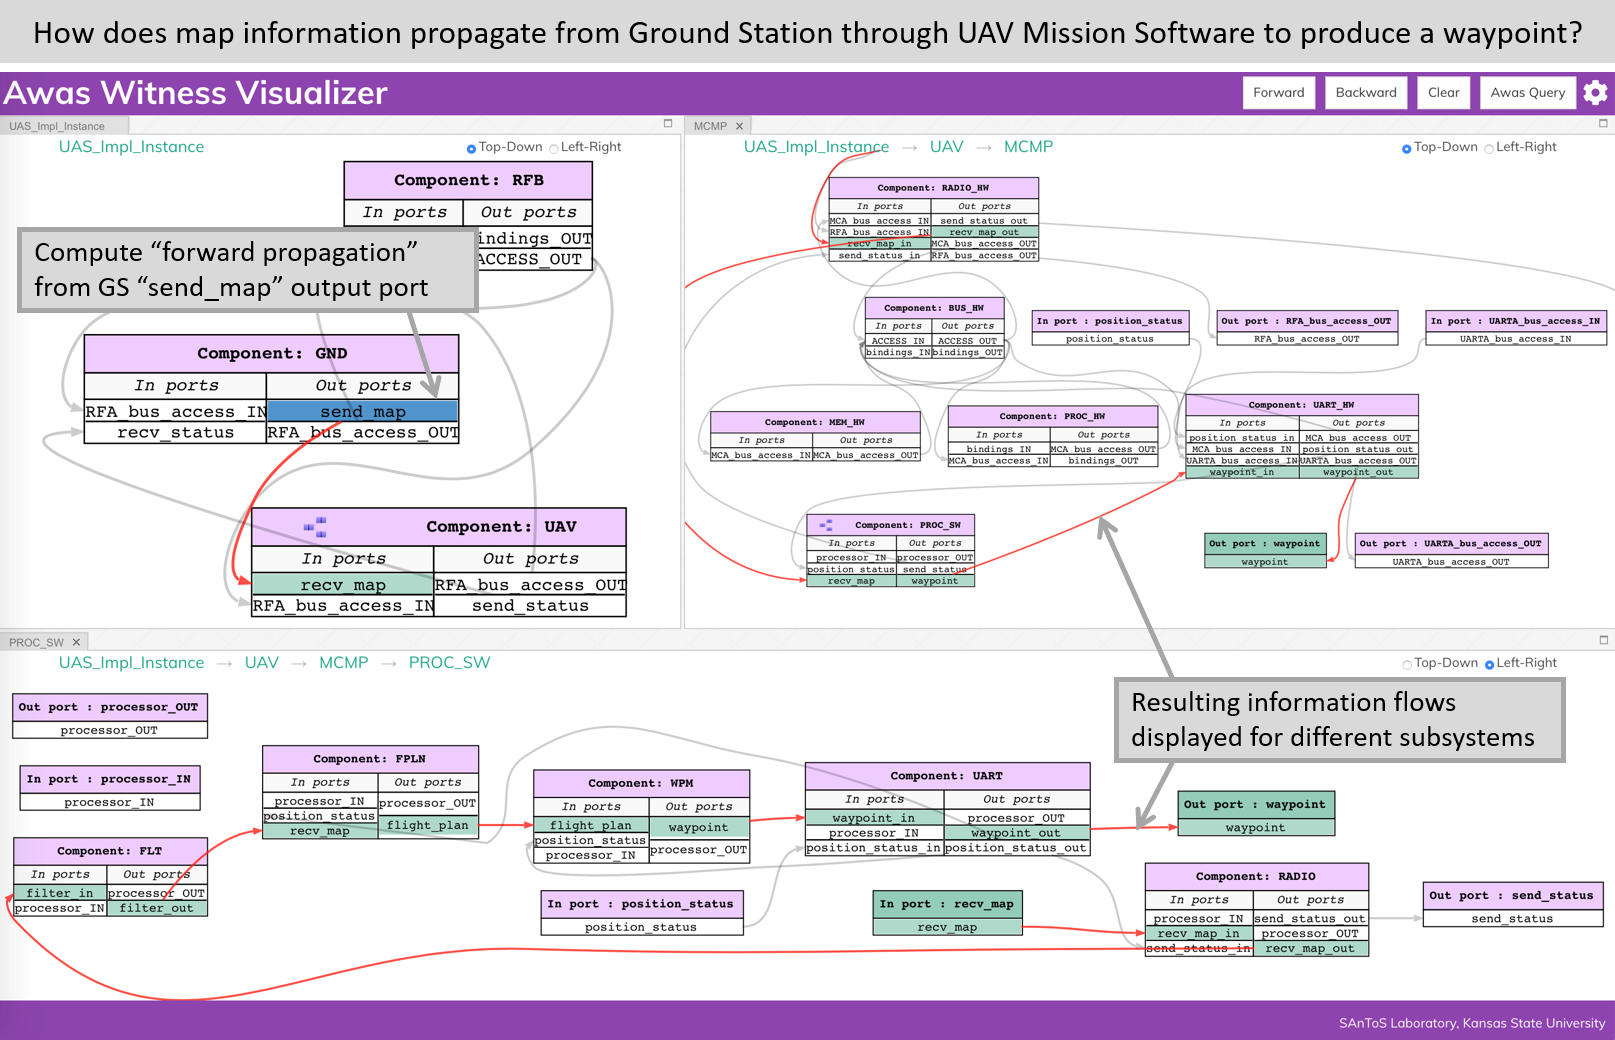
\includegraphics[width=\textwidth]{figs/CASE-Awas.png}
	\caption{Awas Information Flow Analysis.} 
	\label{fig:CASE-Awas} 
\end{figure*}

\figref{fig:CASE-Awas} illustrates an example of Awas information flow reachability analysis.
%From a given component or port (e.g., an output port of the Ground Station),
In our UAV example, Awas can compute and visualize how the information in Ground Station messages flows through the system
as well as the components or ports that may directly or indirectly consume data derived from that information.
Awas supports a number of forms of forward and backward interactive information queries.
Using the Awas script-based query language, one can specify and check more complex properties, e.g.,
that information must flows through specific ports or components.
These end-to-end flow specifications are often useful for supporting verification of the
effectiveness of cyber-resiliency components.   An Awas specification can state that
information from untrusted components such as the Ground Station always flow through the
Attestation Gate and filter components before reaching the Flight Control or other components
that make critical decisions about the flight or mission of the UAV.

%The HAMR code generation and associated formally verified information
%flow correspondence evidence described subsequently
%%%described in Section~\ref{subsec:hamr}
%guarantees that the seL4 microkernel is configured to permit the exact
%inter-component information flows analyzed and visualized by Awas at
%the model level.
